\section{Data-Visualization}

\subsection{Mode Maps}

Mode maps are a common way to visualize the distribution of color terms in a color space (Fig. \ref{fig:mode_prop_maps} middle panel).
These visualizations display the 330 Color chips (Fig. \ref{fig:mode_prop_maps} upper panel) as a two-dimensional map of the color space, where the color of each chip represents the most common color term for that chip.
We innovate here a bit, by improving the standard visualization with the following trick. 
 For each chip, we assign it a color that is the average over all chips in that category.
%We visualize the selected color for each  chip by assigning it to a color which  is the average over all chips of this category.
%In this way the color of each term is calculated by taking the mean of all chips that were assigned to that term, and thus allow us to quickly see the selected visual category over the space of all chips.
 As a result, each term's color is calculated based on the mean of all chips assigned to it, allowing us to quickly see the selected visual category over all chips (See Fig.\ref{fig:mode_prop_maps} lower panel).
This approach is more informative than using generic unrelated colors for example in \cite{regierColor2007} (See Fig.\ref{fig:mode_prop_maps} middle panel). 
% In the case of ties, the term that occurs the most in the overall dataset wins.


%The characters '*' and '+' are used to indicate the proportion of the winning term in respect to the number of the total number of terms assigned to that chip.
%Therefore, they indicate a measure of confidence in the assignment.

\subsection{Proportion Maps}
We propose another new way of visualizing color lexicons and their distribution in color space.
For every chip our proportion maps show the distribution of the first three most common terms (Fig. \ref{fig:mode_prop_maps} lower panel).
This provides additional information and allows a more intuitive understanding of the centers and boundaries of color categories in color space. Importantly, it allows us to see better the overlap and boundary of color categories beyond only the most frequent color. 

% insert image that represents the mode map
% \begin{figure}[htp]
%     \centering
%     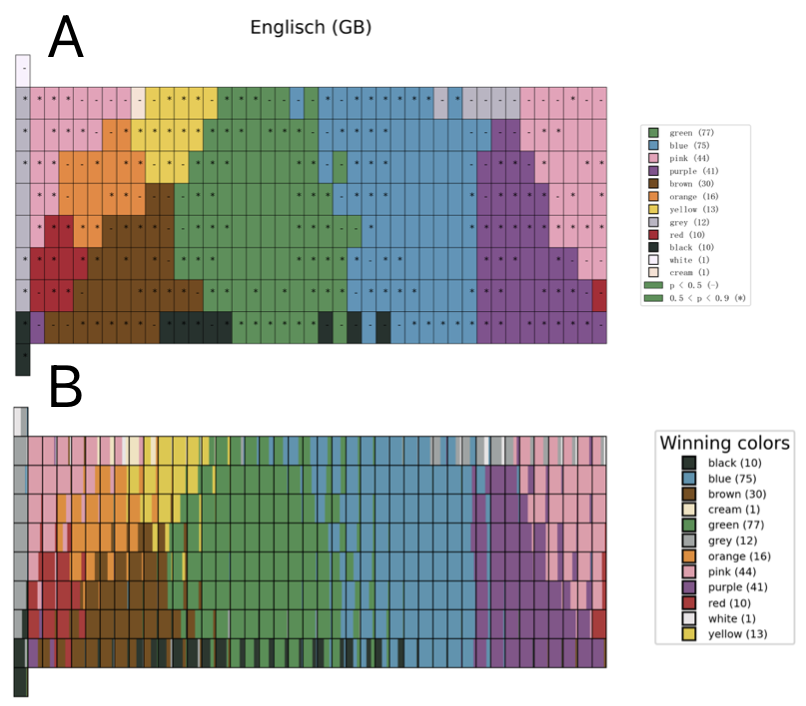
\includegraphics[width=\textwidth]{images/GradientAndMode.png}
%     \caption{Both show the same data we collected for English. A: Mode Map, B: \textit{NAME} map.
%     Mode maps give an overconfident impression about the solidness of  categories and hide much of information between.
%     }
%     \label{fig:maps}
% \end{figure}

\begin{figure}[htbp]
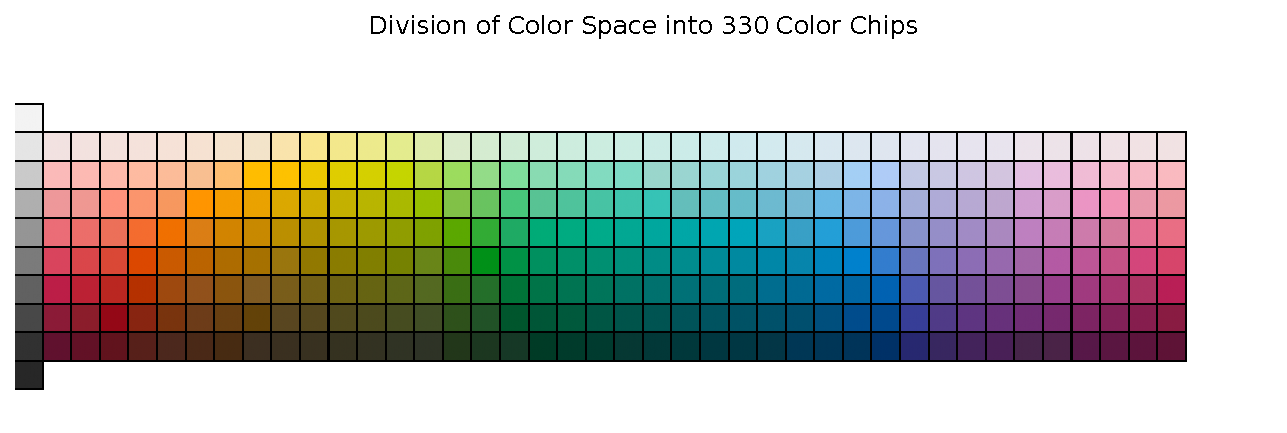
\includegraphics[page=1, width=0.88\linewidth]{images/munsell_chips.pdf}
% 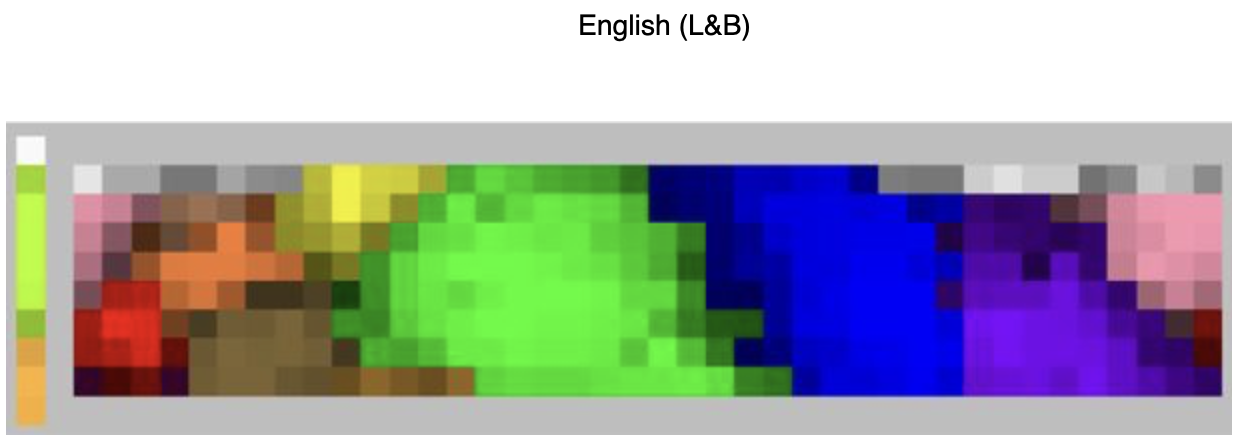
\includegraphics[page=1, width=0.81\linewidth]{images/LnB_generic.png}
% 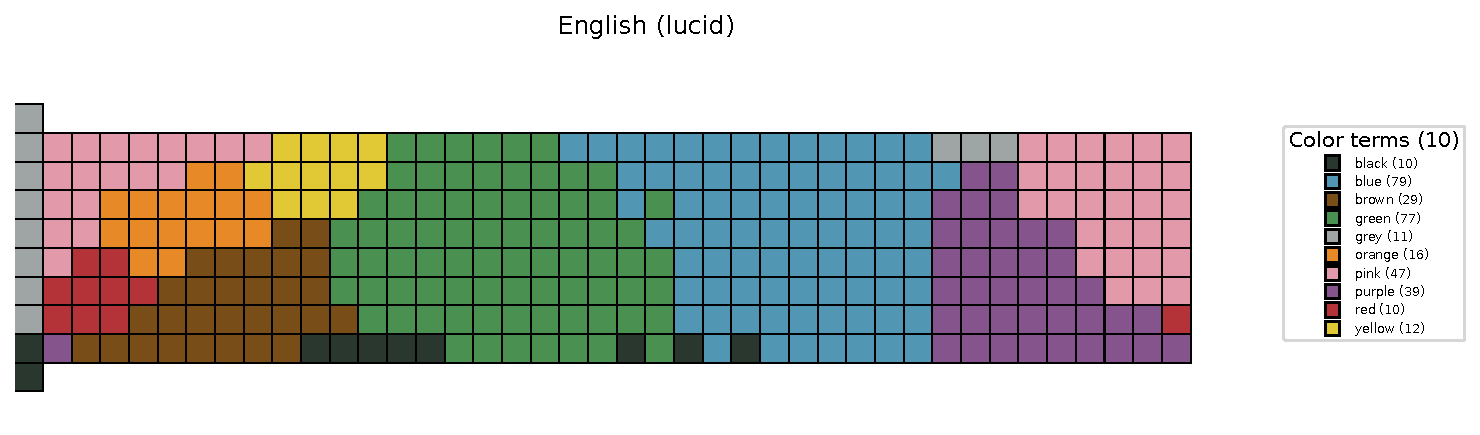
\includegraphics[page=1, width=\linewidth]{images/mode_maps/English (lucid)mode-map.pdf}
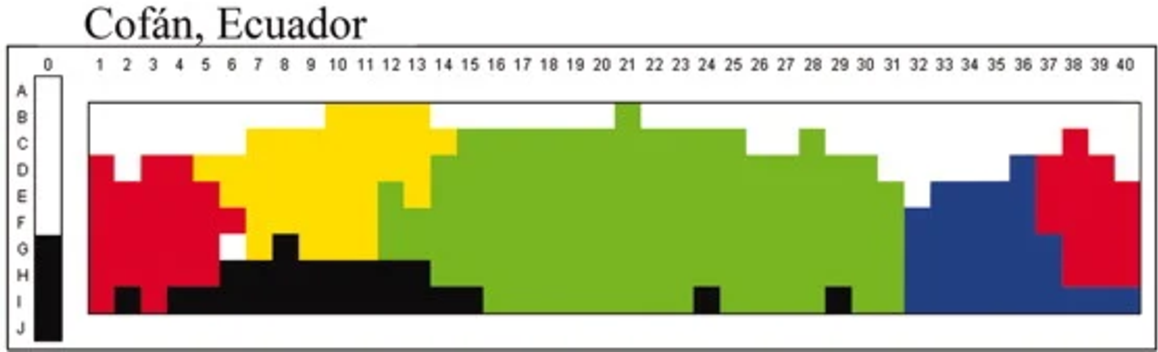
\includegraphics[page=1, width=0.81\linewidth]{images/mode_map.pdf}
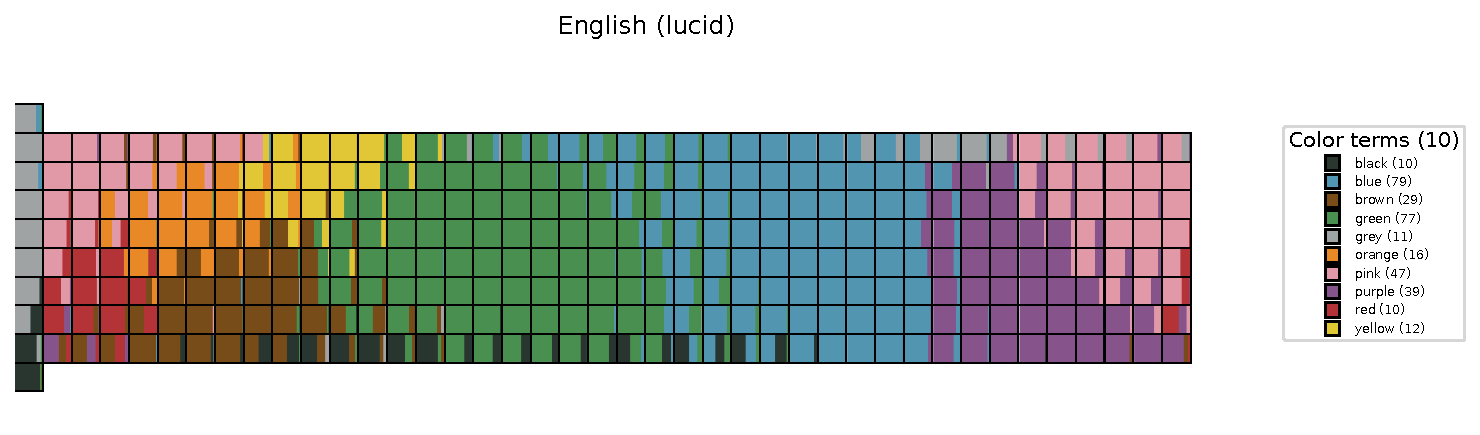
\includegraphics[page=1, width=\linewidth]{images/mode_maps/English (lucid).pdf}
\decoRule
\caption[330 Color Stimuli, Mode Map Regier et al. and Proportion Map]{330 Color Stimuli, Mode Map \parencite{regierColor2007} and Proportion Map. Upper panel: Subdivided color space into 330 color chips analog to the Munsell chips used in the WCS. Middle panel: Mode map of Cofán (Ecuador), a language examined in the WCS. Color naming pattern of six color categories visualized by \textcite{regierColor2007} using generic colors.
Lower panel: Proportional map using the mean RGB values for each color category. For each chip three most common color terms presented, therefore give intuitive information about the consensus for single color chips.}
\label{fig:mode_prop_maps}
\end{figure}